\documentclass[conference]{IEEEtran}
\IEEEoverridecommandlockouts
% --- Packages ---
\usepackage{amsmath,amssymb,amsfonts}
\usepackage{algorithmic}
\usepackage{graphicx}
\usepackage{textcomp}
\usepackage{xcolor}
\usepackage{booktabs}
\usepackage{array}
\def\BibTeX{{\rm B\kern-.05em{\sc i\kern-.025em b}\kern-.08em
    T\kern-.1667em\lower.7ex\hbox{E}\kern-.125emX}}

\begin{document}

\title{FPGA-Based LQR Control Implementation for\\ Quadrotor UAV Stabilization}

\author{\IEEEauthorblockN{Yusuf \"Ozeser}
\IEEEauthorblockA{\textit{Department of Electrical and Electronics Engineering} \\
\textit{Marmara University}\\
Istanbul, T\"urkiye \\
yusufozeser@marun.edu.tr}
}

\maketitle

% ===================== ABSTRACT =====================
\begin{abstract}
This paper presents the design and FPGA-in-the-Loop (FIL) implementation of a Linear Quadratic Regulator (LQR) for the attitude and altitude stabilization of a quadrotor unmanned aerial vehicle (UAV). The nonlinear quadrotor dynamics are linearized about the hover operating point, and an optimal state-feedback gain is computed by solving the algebraic Riccati equation. The controller is described in MATLAB/Simulink using HDL-compatible blocks, converted to a 16-bit fixed-point representation, and synthesized for a low-cost Xilinx Artix-7 (xc7a35t) device on the Basys3 development board through the HDL Workflow Advisor. The implemented controller is validated in FIL execution mode, where the bitstream running on the physical FPGA is driven by the plant model simulated in Simulink and communicates over the JTAG interface. A challenging tilted-takeoff scenario is used, in which the quadrotor starts from large initial roll, pitch, and yaw angles and is commanded to climb to a 30~m altitude. Actuator saturation is included to reflect realistic thrust limits. The FIL results show that the fixed-point FPGA implementation reproduces the floating-point reference response with a negligible, near-zero tracking error, while consuming less than 5\% of the available logic resources of the target device. These results demonstrate that an optimal LQR controller can be deployed on an inexpensive FPGA with negligible loss of accuracy and substantial headroom for additional functionality.
\end{abstract}

\begin{IEEEkeywords}
FPGA, quadrotor, UAV, LQR, optimal control, FPGA-in-the-Loop, fixed-point, Basys3
\end{IEEEkeywords}

% ===================== I. INTRODUCTION =====================
\section{Introduction}
Unmanned aerial vehicles (UAVs), and quadrotors in particular, have become a widely used research and application platform owing to their mechanical simplicity and their ability to achieve full six-degree-of-freedom motion through the variation of four rotor speeds. The quadrotor is, however, an inherently unstable and strongly coupled nonlinear system. Gyroscopic effects, aerodynamic drag, gravity, and inertial cross-coupling all act simultaneously, which makes the design and the real-time execution of its stabilizing controller a demanding task.

A large body of work addresses quadrotor control using classical and modern techniques. Proportional--Integral--Derivative (PID) control remains popular because of its simplicity, short response time, and low steady-state error. Optimal control approaches such as the Linear Quadratic Regulator (LQR) are also attractive because they produce a state-feedback law that minimizes a quadratic cost function balancing tracking performance against control effort, and they handle multi-input multi-output coupling in a single systematic framework. Regardless of the control law, practical deployment requires a computing platform capable of evaluating the controller at a high update rate with deterministic timing.

Field Programmable Gate Arrays (FPGAs) are well suited to this requirement. Their inherent parallelism and high clock frequency allow control computations to be executed concurrently with deterministic latency, in contrast to sequential software running on a general-purpose processor with operating-system overhead. This advantage has motivated several FPGA-based implementations of optimal and intelligent controllers, including hardware realizations of LQR-based observers and PID controllers for UAV stabilization.

The FPGA-in-the-Loop (FIL) methodology offers a particularly convenient path from model to hardware. In FIL, the controller is synthesized and programmed onto a physical FPGA, while the plant and the reference generator continue to run in simulation. The two communicate at every sample, so the designer can verify the behavior of the actual hardware bitstream against the validated floating-point model before any flight test, and without writing hand-coded HDL.

This work is inspired by the FPGA-based PID approach of Khati \textit{et al.}~[1], who implemented four PID controllers for quadrotor stabilization on a Zybo Zynq-7000 board using HDL Coder and the FIL workflow. The present paper follows the same overall methodology but differs in two important respects. First, the PID control law is replaced by an optimal LQR state-feedback controller, which captures the cross-coupling of the quadrotor in a single multivariable gain matrix instead of four independent single-loop controllers. Second, the target hardware is changed from the Zynq-7000 platform to a low-cost, logic-only Xilinx Artix-7 device (xc7a35t) on the Basys3 board, demonstrating that the optimal controller fits comfortably within an inexpensive FPGA. In addition, this work introduces explicit actuator saturation modeling and a challenging tilted-takeoff initial condition to exercise the controller under realistic and demanding conditions.

The remainder of the paper is organized as follows. Section~II develops the nonlinear dynamic model of the quadrotor using the Euler--Newton formulation. Section~III presents the linearization and the LQR design. Section~IV describes the FIL implementation, including the HDL code generation, the fixed-point conversion, and the synthesis for the Basys3 board. Section~V reports the FIL simulation results and the FPGA resource utilization. Section~VI concludes the paper.

% ===================== II. DYNAMIC MODEL =====================
\section{Dynamic Model of the Quadrotor}
The quadrotor is modeled as a rigid body of mass $m$ subject to the thrust and drag of its four rotors, gravity, and aerodynamic friction. Two reference frames are used: an inertial earth-fixed frame and a body-fixed frame attached to the vehicle's center of mass. The vehicle position in the inertial frame is denoted $\zeta = [x\ y\ z]^{T}$, and its orientation is described by the three Euler angles roll $\phi$, pitch $\theta$, and yaw $\psi$. The four rotors generate individual thrust forces $F_i = b\,\omega_i^{2}$, where $\omega_i$ is the angular speed of the $i$-th rotor and $b$ is the thrust coefficient, and a reactive drag torque proportional to the drag coefficient $d$.

\subsection{Force and Moment Generation}
Following the Euler--Newton formulation, the rigid-body motion is governed by the balance of forces and moments expressed in the body frame. The translational dynamics combine the total rotor thrust $F_f$, the gravitational force $F_g$, and the translational aerodynamic drag $F_t$, while the rotational dynamics combine the moment $M_f$ produced by the differential rotor thrust and drag with the aerodynamic friction moment $M_a$:
\begin{align}
m\ddot{\zeta} &= F_f + F_g + F_t,\\
J\dot{\Omega} &= M_f - \Omega \times J\Omega + M_a,
\end{align}
where $\Omega = [\dot\phi\ \dot\theta\ \dot\psi]^{T}$ is the angular velocity vector and $J = \mathrm{diag}(I_x, I_y, I_z)$ is the diagonal inertia matrix of the symmetric airframe. The term $\Omega \times J\Omega$ captures the gyroscopic and inertial cross-coupling between the three rotational axes. The four physical rotor commands are mapped to one collective thrust and three body torques through the standard control-allocation relation, so that the control vector consists of the total thrust $u_1$ along the body $z$-axis and the roll, pitch, and yaw torques $u_2$, $u_3$, $u_4$.

\subsection{Equations of Motion}
The model parameters used in this work are summarized in Table~\ref{tab:params}. The mass, inertias, arm length, and thrust and drag coefficients follow the reference quadrotor~[1]. The aerodynamic friction coefficients $K_{2x}$, $K_{2y}$, $K_{2z}$ associated with the angular-rate damping are taken to be equal to the corresponding translational drag coefficients for the purposes of this simulation, as their precise values have a negligible effect on the closed-loop response, which is dominated by the optimal feedback gain and the actuator saturation.

\begin{table}[!t]
\renewcommand{\arraystretch}{1.3}
\caption{Quadrotor Model Parameters}
\label{tab:params}
\centering
\begin{tabular}{llll}
\toprule
\textbf{Parameter} & \textbf{Symbol} & \textbf{Value} & \textbf{Unit}\\
\midrule
Mass & $m$ & 0.65 & kg\\
Gravitational acceleration & $g$ & 9.81 & m/s$^2$\\
Arm length & $l$ & 0.23 & m\\
Roll/pitch inertia & $I_x=I_y$ & $7.5\times10^{-3}$ & kg$\cdot$m$^2$\\
Yaw inertia & $I_z$ & $1.3\times10^{-2}$ & kg$\cdot$m$^2$\\
Thrust coefficient & $b$ & $3.13\times10^{-5}$ & --\\
Drag coefficient & $d$ & $7.5\times10^{-7}$ & --\\
Altitude damping & $K_{1z}$ & $6.354\times10^{-4}$ & --\\
Ang.-rate damping (roll, pitch) & $K_{2x}\!=\!K_{2y}$ & $5.56\times10^{-4}$ & --\\
Ang.-rate damping (yaw) & $K_{2z}$ & $6.354\times10^{-4}$ & --\\
\bottomrule
\end{tabular}
\end{table}

Expanding the force and moment balance and retaining the altitude and attitude subsystem that is relevant for stabilization, the scalar equations of motion are obtained as:
\begin{align}
\ddot{z} &= -g + \frac{\cos\phi\cos\theta}{m}\,u_1 - \frac{K_{1z}}{m}\dot{z}\\[2pt]
\ddot{\phi} &= \frac{I_y - I_z}{I_x}\dot{\theta}\dot{\psi} - \frac{K_{2x}}{I_x}\dot{\phi} + \frac{1}{I_x}u_2\\[2pt]
\ddot{\theta} &= \frac{I_z - I_x}{I_y}\dot{\phi}\dot{\psi} - \frac{K_{2y}}{I_y}\dot{\theta} + \frac{1}{I_y}u_3\\[2pt]
\ddot{\psi} &= \frac{I_x - I_y}{I_z}\dot{\phi}\dot{\theta} - \frac{K_{2z}}{I_z}\dot{\psi} + \frac{1}{I_z}u_4
\end{align}

Here $u_1$ is the total thrust along the body $z$-axis, and $u_2$, $u_3$, $u_4$ are the roll, pitch, and yaw control torques, respectively. The terms containing products of the angular rates represent the gyroscopic and inertial cross-coupling between the rotational axes, and the terms containing $K_{1z}$, $K_{2x}$, $K_{2y}$, $K_{2z}$ represent the translational and aerodynamic friction, modeled here as linear (viscous) damping in the angular rates. The rotor gyroscopic effects associated with the net rotor speed are neglected, since they vanish at the hover linearization point about which the controller is designed.

For control design, the state vector is defined as
\begin{equation}
x = \begin{bmatrix} z & \dot{z} & \phi & \dot{\phi} & \theta & \dot{\theta} & \psi & \dot{\psi} \end{bmatrix}^{T},
\end{equation}
which gives an eight-dimensional state with four control inputs $u = [u_1\ u_2\ u_3\ u_4]^{T}$. This choice retains the altitude channel and the three attitude channels, which are the degrees of freedom directly actuated by the collective thrust and the body torques. The horizontal translational dynamics ($x$ and $y$) are driven indirectly through the attitude and are not included in the stabilization model, as the objective of this work is altitude tracking together with attitude stabilization.

% ===================== III. LQR DESIGN =====================
\section{LQR Control Design}
\subsection{Linearization}
The dynamic model is nonlinear because of the trigonometric terms in the thrust projection and the products of angular rates in the rotational equations. To apply linear optimal control, the model is linearized about the hover operating point, at which all angles, all velocities, and all angular rates are zero and the thrust balances gravity. At this point the thrust projection $\cos\phi\cos\theta \approx 1$ and all the rate-product terms vanish, so the model reduces to a linear time-invariant system
\begin{equation}
\dot{x} = Ax + Bu.
\end{equation}
The hover thrust required to balance the weight is
\begin{equation}
u_{1,\text{hover}} = mg = 6.3765~\text{N},
\end{equation}
which is added back as a constant offset after the linear control law is computed, so that the LQR operates on the deviation from hover.

\subsection{Optimal Gain Computation}
The LQR minimizes the infinite-horizon quadratic cost
\begin{equation}
J = \int_0^{\infty} \left( x^{T} Q x + u^{T} R u \right) dt,
\end{equation}
where $Q \succeq 0$ penalizes the state deviation and $R \succ 0$ penalizes the control effort. The optimal state-feedback gain is
\begin{equation}
u = -Kx, \qquad K = R^{-1} B^{T} P,
\end{equation}
where $P$ is the symmetric positive-definite solution of the algebraic Riccati equation
\begin{equation}
A^{T} P + P A - P B R^{-1} B^{T} P + Q = 0.
\end{equation}
The weighting matrices were selected to give a smooth, realistic closed-loop response without excessive control demand:
\begin{align}
Q &= \text{diag}(1,\ 2,\ 5,\ 1,\ 5,\ 1,\ 5,\ 1),\\
R &= \text{diag}(0.1,\ 1,\ 1,\ 1).
\end{align}
The relatively low altitude-position weight ($Q_{1,1}=1$) was chosen deliberately; a larger weight produced an aggressive climb with significant overshoot, whereas the selected value yields a monotonic, overshoot-free ascent once actuator saturation is applied.

Because the linearized altitude and attitude subsystems are decoupled at hover, the resulting gain matrix $K$ is block-diagonal with the structure
\begin{equation}
K = \begin{bmatrix}
3.1623 & 4.9097 & 0 & 0 & 0 & 0 & 0 & 0 \\
0 & 0 & 2.2361 & 1.0161 & 0 & 0 & 0 & 0 \\
0 & 0 & 0 & 0 & 2.2361 & 1.0161 & 0 & 0 \\
0 & 0 & 0 & 0 & 0 & 0 & 2.2361 & 1.0280
\end{bmatrix}.
\end{equation}
Each row maps one control channel to its corresponding position and velocity states: the first row controls altitude through $z$ and $\dot{z}$, and the remaining three rows control roll, pitch, and yaw through their respective angle and angular-rate states.

\subsection{Actuator Saturation}
A distinguishing feature of this work is the explicit modeling of actuator saturation, which is absent in the reference PID implementation. In a physical quadrotor the electronic speed controllers and motors limit the achievable thrust, so the unbounded output of an idealized controller is not realizable. To capture this, saturation blocks are placed \emph{outside} the LQR subsystem, on the pure-Simulink side of the model, so that only the controller itself is synthesized to hardware while the physical actuator limit is enforced by the plant interface, as it would be in reality.

The total thrust is limited to approximately 20~N, corresponding to a thrust-to-weight ratio of about 3, which is typical for a small quadrotor. Since the total thrust is the sum of the LQR output and the hover offset,
\begin{equation}
u_{1,\text{total}} = u_{1,\text{LQR}} + mg,
\end{equation}
the LQR contribution is bounded to $[-6.38,\ +13.62]$~N so that the total thrust stays within $[0,\ 20]$~N. The control torques are limited to $\pm 0.5$~N$\cdot$m, which provides a safe margin above the torque available from the differential thrust of the four rotors.

% ===================== IV. FIL IMPLEMENTATION =====================
\section{FPGA-in-the-Loop Implementation}
\subsection{Design Flow}
The complete design flow is carried out within MATLAB/Simulink and the HDL Coder toolchain, eliminating the need for hand-written HDL. The LQR control law is built as a Simulink subsystem using only blocks supported by HDL Coder. The plant model, the hover-thrust offset, the actuator saturation, and the reference generator remain on the pure-Simulink side of the model and are not synthesized to hardware. This separation ensures that the FPGA implements exactly the controller and nothing else, which keeps the hardware footprint minimal and the validation clean. The overall closed-loop model used for the FIL test is shown in Fig.~\ref{fig:model}.

\begin{figure}[!t]
\centering
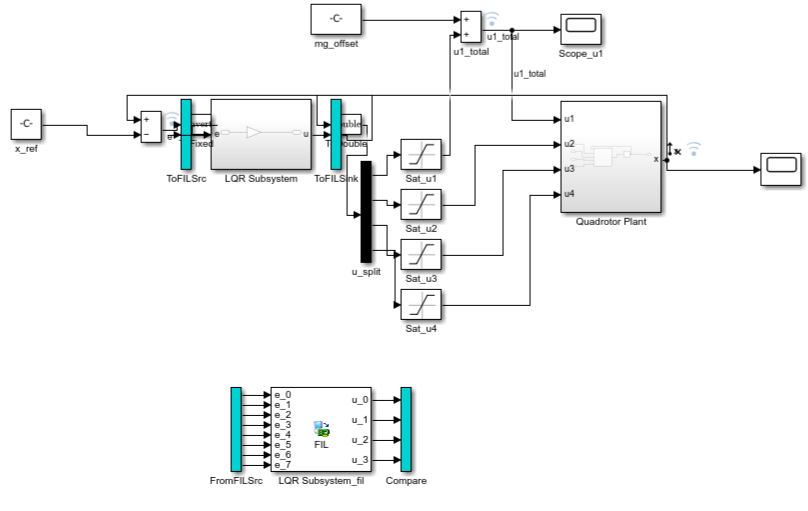
\includegraphics[width=\columnwidth]{figs/fig_model.png}
\caption{Simulink model used for the FPGA-in-the-Loop test. The LQR subsystem (synthesized to the FPGA) is bracketed by fixed-point conversion blocks; the hover-thrust offset, the actuator saturation blocks (Sat\_u1--Sat\_u4), and the quadrotor plant remain on the pure-Simulink side.}
\label{fig:model}
\end{figure}

The HDL Workflow Advisor was configured for the FPGA-in-the-Loop target workflow with the Basys3 board, the Xilinx Vivado synthesis tool, and a target frequency of 50~MHz. VHDL was selected as the target language. The workflow proceeds through target selection, model preparation and compatibility checking, HDL code generation, and finally the FIL build, which synthesizes the design, runs implementation, writes the bitstream, and generates the FIL test harness automatically.

\subsection{Fixed-Point Conversion}
FPGA fabric does not natively support floating-point arithmetic in an area-efficient way, so the floating-point controller was converted to a fixed-point representation. A 16-bit word length was used throughout the controller datapath. Because the altitude reference in this work is 30~m---substantially larger than a typical attitude-only stabilization scenario---the fixed-point ranges had to be widened relative to a small-signal design to prevent wrap-around of the internal signals. The fractional lengths were chosen to give the dynamic ranges listed in Table~\ref{tab:fixedpoint}.

\begin{table}[!t]
\renewcommand{\arraystretch}{1.3}
\caption{Fixed-Point Data Types in the LQR Datapath}
\label{tab:fixedpoint}
\centering
\begin{tabular}{lll}
\toprule
\textbf{Signal} & \textbf{Data type} & \textbf{Approx. range}\\
\midrule
Input conversion (ToFixed) & fixdt(1,16,8) & $\pm128$\\
Error signal $e$ & fixdt(1,16,8) & $\pm128$\\
LQR gain product & fixdt(1,16,6) & $\pm512$\\
Control output $u$ & fixdt(1,16,6) & $\pm512$\\
\bottomrule
\end{tabular}
\end{table}

This widened scaling is necessary specifically because of the large altitude command; a narrower fixed-point format that is adequate for small-angle attitude regulation would saturate or wrap when the altitude error reaches tens of meters.

\subsection{Hardware Target and FIL Setup}
The target device is the Xilinx Artix-7 xc7a35t-cpg236-1 on the Basys3 board. Communication between MATLAB/Simulink and the FPGA takes place over the JTAG interface. After synthesis and implementation, HDL Coder produces the programming bitstream and an automatically generated FIL test model. In this model, the synthesized controller running on the physical FPGA is exercised in parallel with the original floating-point controller, and the two outputs are compared sample by sample. The plant model, driven by the FPGA controller output, closes the loop in simulation while the controller itself executes in real hardware.

% ===================== V. RESULTS =====================
\section{Results and Discussion}
\subsection{Simulation Scenario}
The closed-loop system was evaluated over a 15-second simulation with a fixed step size of 1~ms (15\,001 samples). A deliberately challenging initial condition was used: the quadrotor starts from a tilted attitude with roll $\phi_0 = 0.6$~rad, pitch $\theta_0 = 0.5$~rad, and yaw $\psi_0 = 0.35$~rad, all at zero angular rate, and at zero altitude. The reference commands a climb to $z_{\text{ref}} = 30$~m while driving all three attitude angles back to zero. This tilted-takeoff scenario is more demanding than a near-hover regulation test because the controller must simultaneously reject large initial attitude errors and execute a large altitude maneuver.

\subsection{Closed-Loop Response}
The FIL closed-loop response is summarized in Table~\ref{tab:metrics} and discussed below.

\begin{table}[!t]
\renewcommand{\arraystretch}{1.3}
\caption{Key Performance Metrics (FIL)}
\label{tab:metrics}
\centering
\begin{tabular}{ll}
\toprule
\textbf{Metric} & \textbf{Value}\\
\midrule
Final altitude & 30.0042~m\\
Maximum altitude & 30.0042~m\\
Altitude overshoot & none\\
Peak vertical velocity & 14.86~m/s\\
Peak total thrust $u_1$ & 19.9965~N\\
Final total thrust $u_1$ & 6.36~N\\
Final roll $\phi$ & 0.0002~rad\\
Final pitch $\theta$ & 0.0012~rad\\
Final yaw $\psi$ & 0.0019~rad\\
\bottomrule
\end{tabular}
\end{table}

The altitude rises monotonically from 0 to the 30~m reference and settles within approximately 5--6 seconds with \textbf{no overshoot}, as shown in Fig.~\ref{fig:altitude}. The absence of overshoot is a direct consequence of the actuator saturation: the thrust command reaches its 20~N limit during the climb, which forces the controller to increase altitude gradually rather than with an aggressive, overshooting transient. The maximum altitude equals the final altitude (30.0042~m), confirming that the response never exceeds the reference. The steady-state error is on the order of millimeters, which is negligible for practical flight. The corresponding vertical velocity, shown in Fig.~\ref{fig:zdot}, rises to a peak of about 14.86~m/s during the climb and returns smoothly to zero as the vehicle settles at the commanded altitude.

\begin{figure}[!t]
\centering
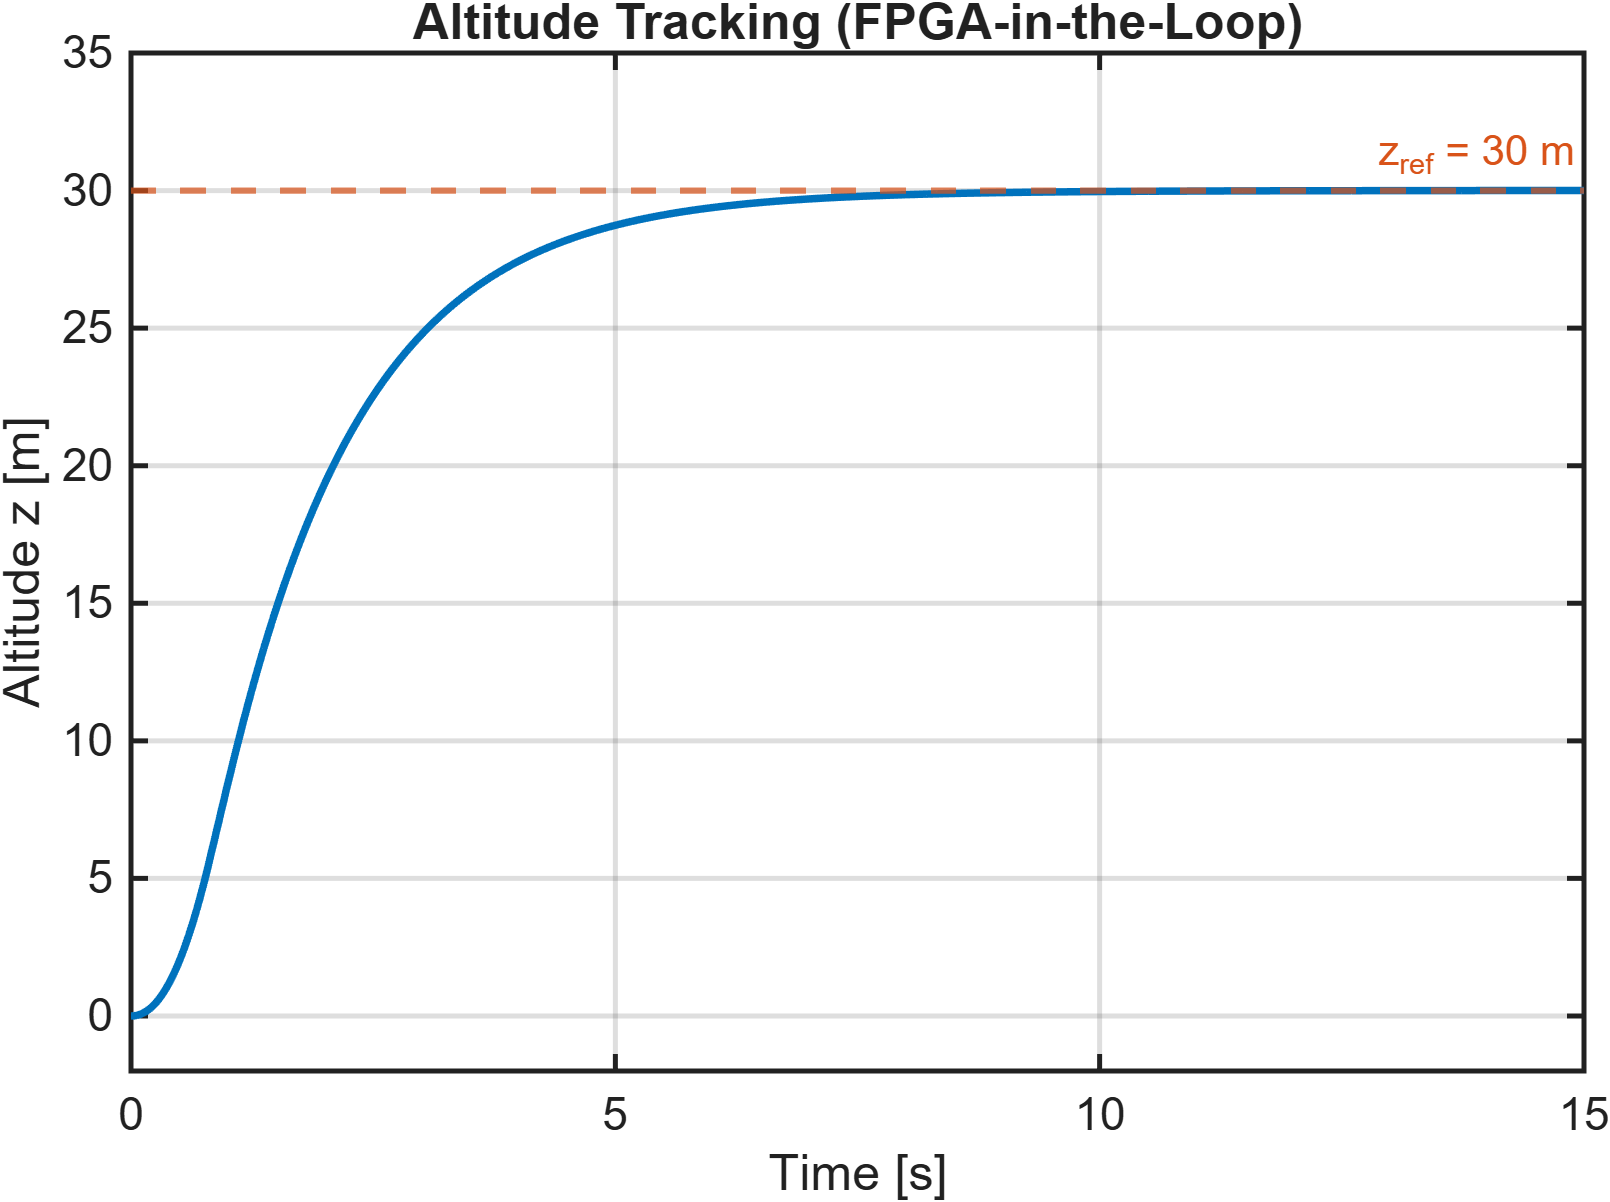
\includegraphics[width=\columnwidth]{figs/fig1_altitude.png}
\caption{Altitude tracking under the FPGA-in-the-Loop LQR controller. The vehicle climbs monotonically to the 30~m reference with no overshoot.}
\label{fig:altitude}
\end{figure}

\begin{figure}[!t]
\centering
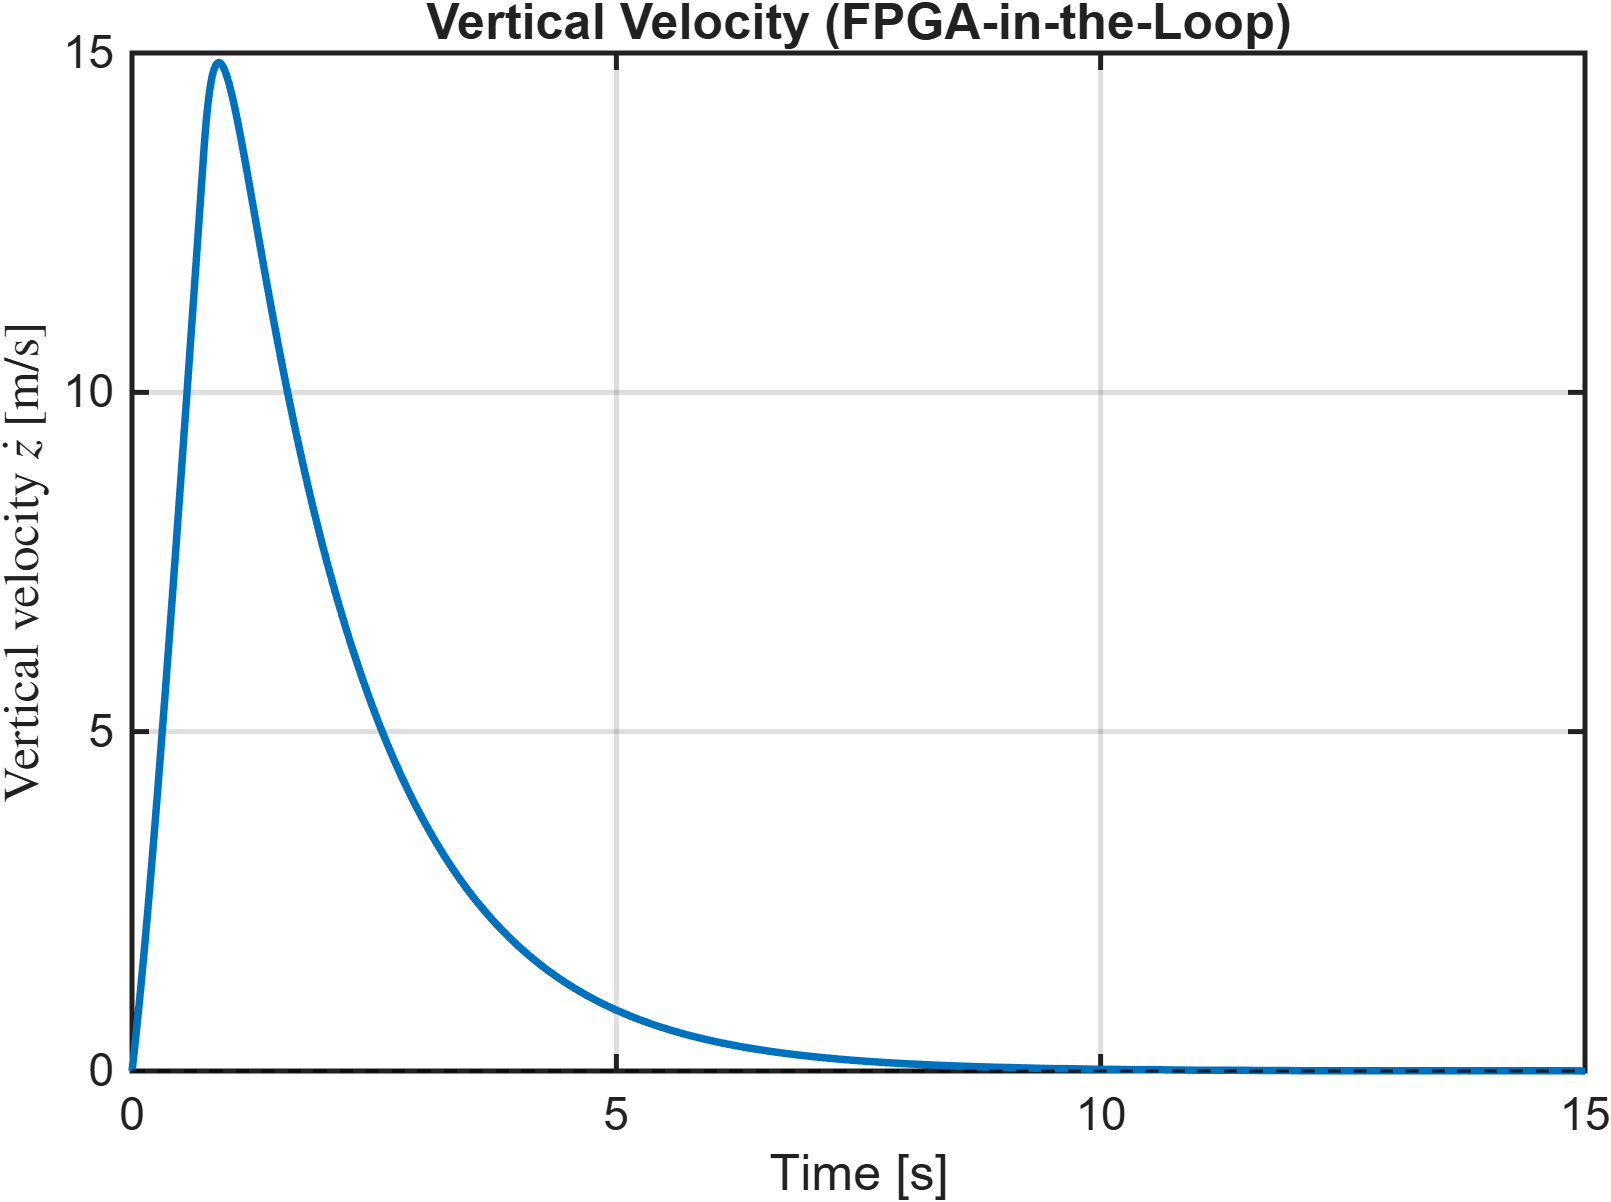
\includegraphics[width=\columnwidth]{figs/fig2_zdot.png}
\caption{Vertical velocity during the climb. The velocity peaks at approximately 14.86~m/s and returns to zero as the altitude settles.}
\label{fig:zdot}
\end{figure}

The three attitude angles converge from their large initial values to within a few thousandths of a radian of zero in well under one second, as shown in Fig.~\ref{fig:attitude}, demonstrating that the LQR rejects the tilted initial condition rapidly while the slower altitude maneuver proceeds. The associated angular velocities, shown in Fig.~\ref{fig:angvel}, exhibit a brief transient peak as the controller arrests the initial tilt and then decay smoothly to zero; the small staircase pattern visible in this trace reflects the quantization of the fixed-point control output, which has no observable effect on the converged response. The final total thrust settles at 6.36~N, essentially equal to the hover thrust $mg = 6.38$~N, as expected for steady-state hover at the commanded altitude. As shown in Fig.~\ref{fig:thrust}, the peak total thrust of 19.9965~N touches the 20~N saturation limit without exceeding it, confirming that the saturation model is active and correctly bounded; the thrust then dips as the vehicle decelerates toward the reference and recovers to the hover value.

\begin{figure}[!t]
\centering
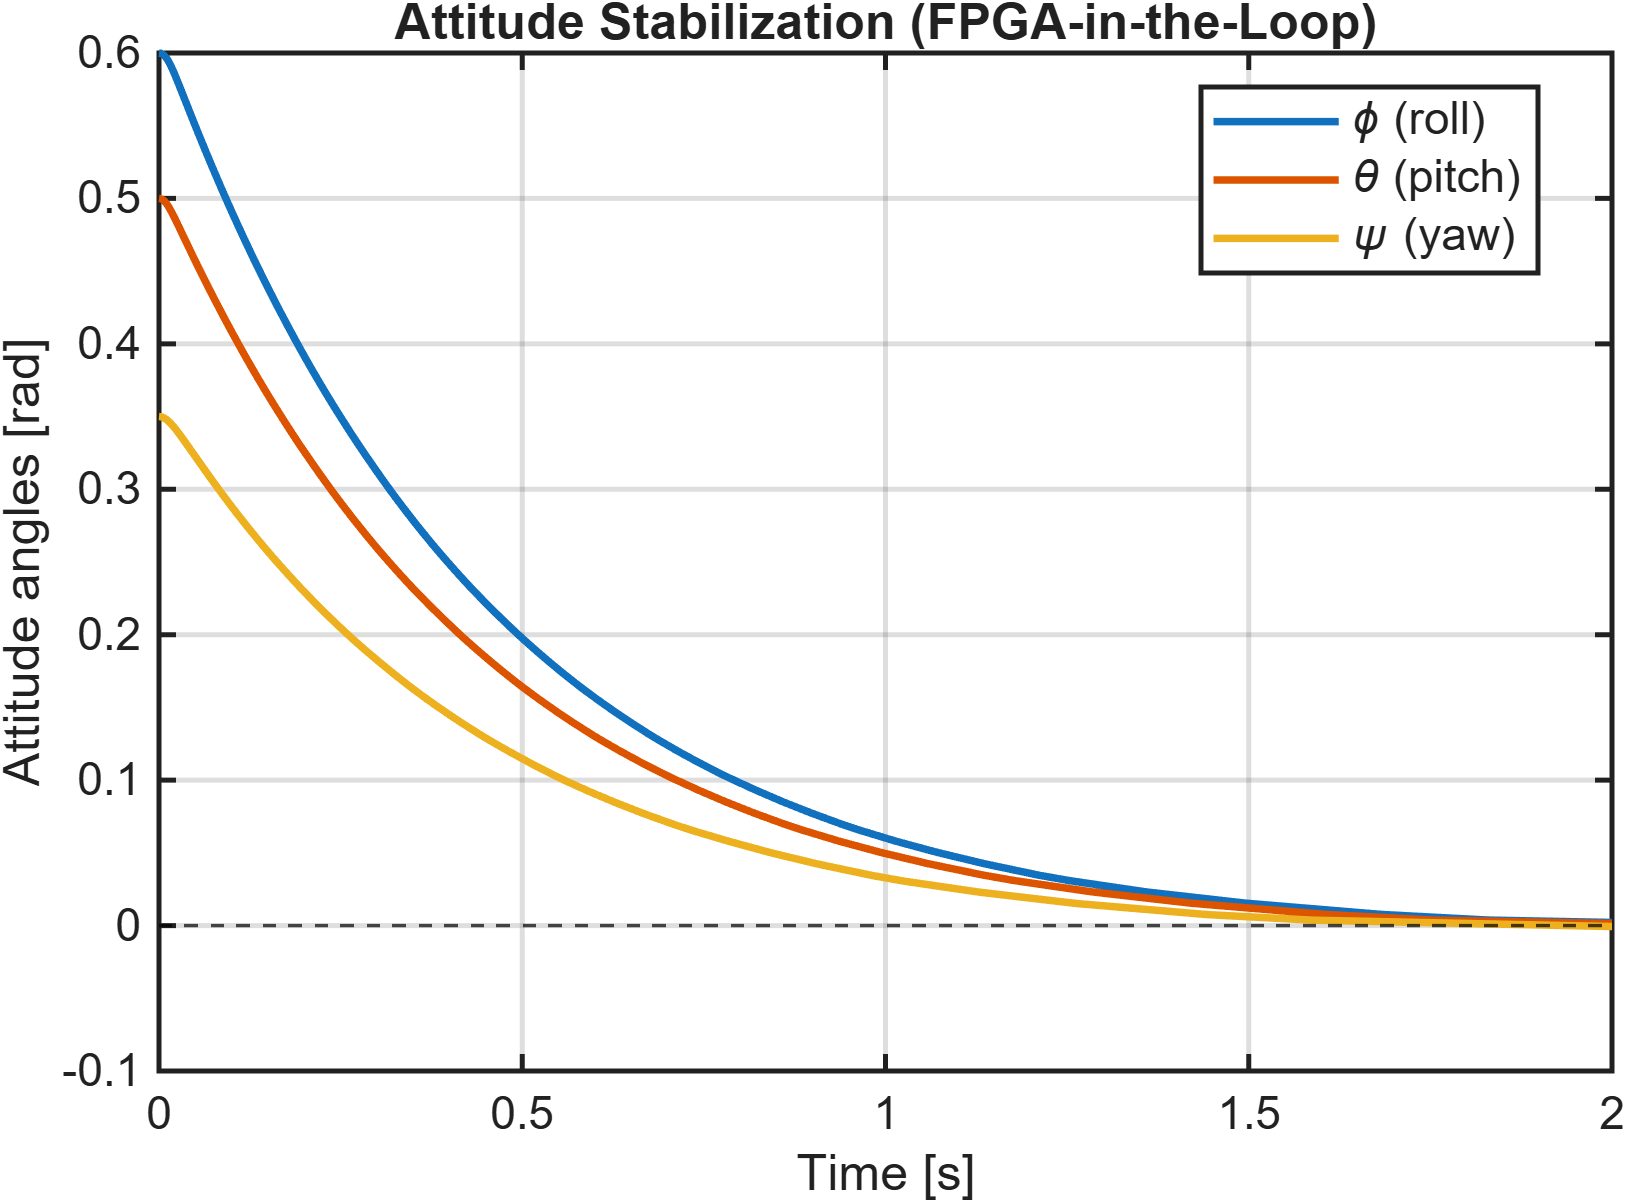
\includegraphics[width=\columnwidth]{figs/fig3_attitude.png}
\caption{Attitude stabilization. The roll, pitch, and yaw angles converge from the tilted initial condition ($\phi_0=0.6$, $\theta_0=0.5$, $\psi_0=0.35$~rad) to near zero in under one second.}
\label{fig:attitude}
\end{figure}

\begin{figure}[!t]
\centering
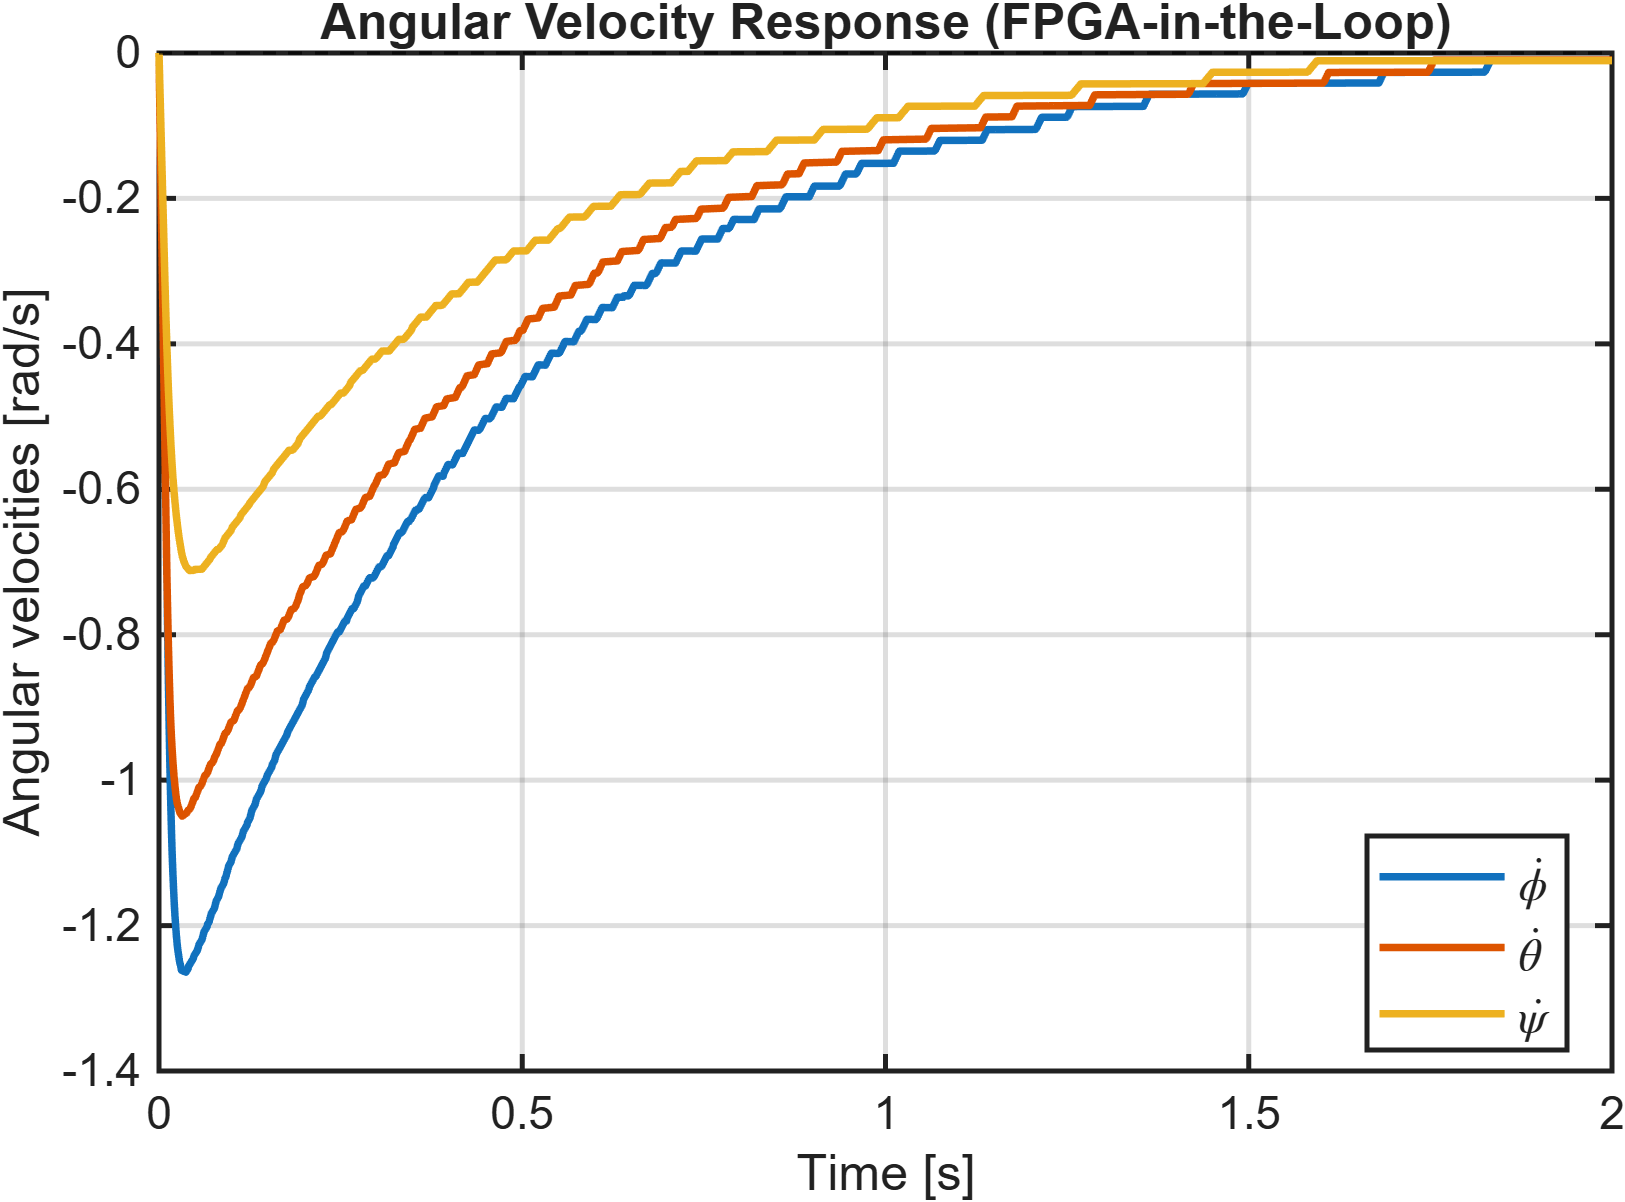
\includegraphics[width=\columnwidth]{figs/fig4_angular_velocities.png}
\caption{Angular velocity response. A brief transient arrests the initial tilt before the rates decay to zero. The staircase pattern reflects the fixed-point quantization of the control output.}
\label{fig:angvel}
\end{figure}

\begin{figure}[!t]
\centering
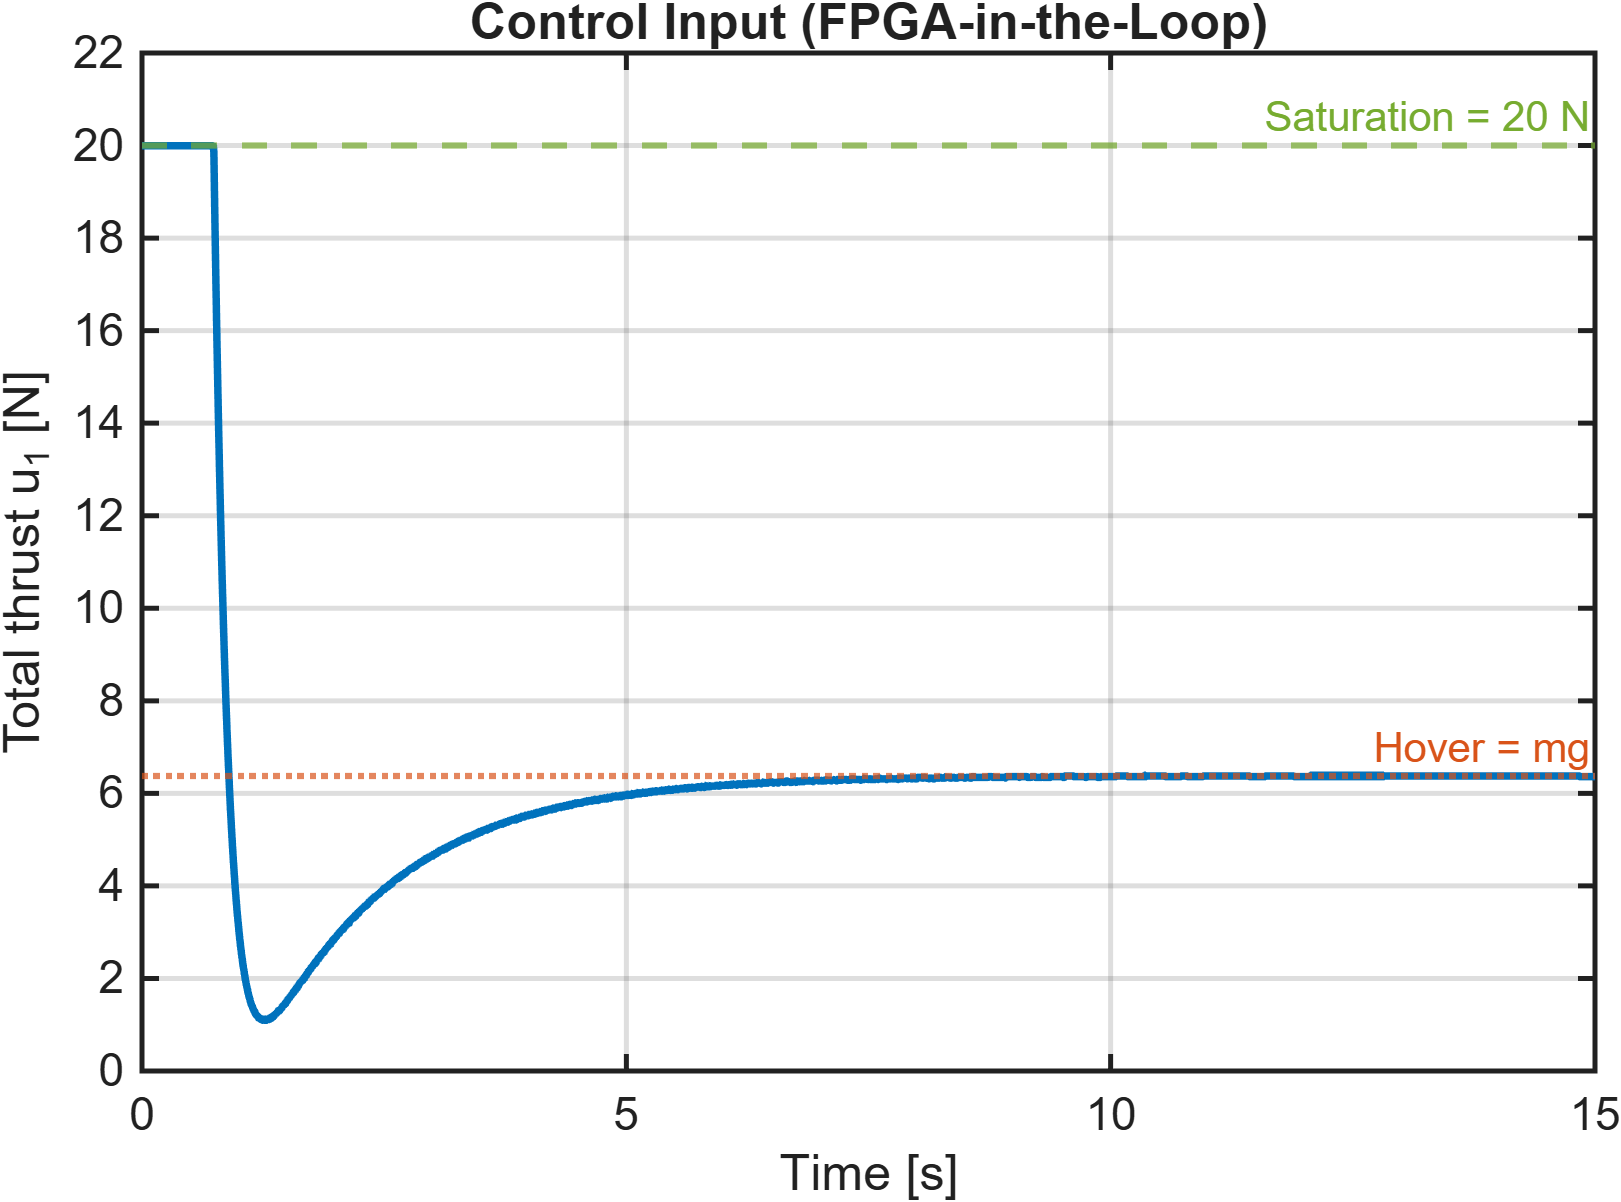
\includegraphics[width=\columnwidth]{figs/fig5_u1_thrust.png}
\caption{Total thrust command $u_1$. The thrust saturates at the 20~N limit during the climb and recovers to the hover value $mg=6.38$~N at steady state.}
\label{fig:thrust}
\end{figure}

\subsection{Hardware Validation}
The central result of the FIL test is the comparison between the controller executing on the physical FPGA and the floating-point reference controller. Across all 15\,001 samples, the difference between the FPGA output and the reference output remains negligible: the error trace stays essentially flat at zero throughout the simulation, with deviations small enough to have no practical effect on the closed-loop response. This near-zero agreement confirms that the 16-bit fixed-point implementation, with the widened scaling described in Section~IV-B, preserves the optimal control behavior to within a negligible margin. In other words, the controller running in real hardware reproduces the floating-point design with an accuracy that is more than sufficient for the stabilization task.

\subsection{FPGA Resource Utilization}
The post-implementation resource utilization of the synthesized LQR controller on the xc7a35t device is reported in Table~\ref{tab:util}.

\begin{table}[!t]
\renewcommand{\arraystretch}{1.3}
\caption{FPGA Resource Utilization (xc7a35t, Post-Implementation)}
\label{tab:util}
\centering
\begin{tabular}{lrrr}
\toprule
\textbf{Resource} & \textbf{Used} & \textbf{Available} & \textbf{Util.}\\
\midrule
Slice LUTs & 929 & 20\,800 & 4.47\%\\
Slice Registers (FF) & 1\,229 & 41\,600 & 2.95\%\\
Block RAM & 5.5 & 50 & 11.00\%\\
DSP48E1 & 8 & 90 & 8.89\%\\
Bonded IOB & 1 & 106 & 0.94\%\\
BUFG & 3 & 32 & 9.38\%\\
MMCM & 1 & 5 & 20.00\%\\
\bottomrule
\end{tabular}
\end{table}

The controller is extremely compact. Logic resources---the LUTs and flip-flops that implement the control arithmetic and the surrounding control logic---remain below 5\% of the device, and only 8 of the 90 DSP slices are used to perform the multiply-accumulate operations of the state-feedback gain matrix. The block RAM usage arises primarily from the FIFO buffers of the JTAG-based FIL communication interface rather than from the controller itself, and the single MMCM provides the clock for the design. The very low logic and DSP utilization shows that an optimal multivariable LQR controller fits comfortably on a low-cost FPGA with the overwhelming majority of the fabric still free, leaving ample room to integrate additional functionality such as state estimation, sensor interfaces, or multiple controllers on the same device.

It is worth noting that the structure of the synthesized hardware depends on the controller architecture---the dimensions of the gain matrix and the fixed-point word lengths---rather than on the specific numerical gain values. Re-tuning the LQR weights changes the entries of $K$ but not the synthesized datapath, so the resource utilization in Table~\ref{tab:util} is representative of this controller class regardless of the particular weighting chosen.

% ===================== VI. CONCLUSION =====================
\section{Conclusion}
This paper presented the design and FPGA-in-the-Loop implementation of an LQR controller for quadrotor attitude and altitude stabilization on a low-cost Xilinx Artix-7 (xc7a35t) device. The nonlinear quadrotor model was linearized about hover, an optimal state-feedback gain was obtained by solving the algebraic Riccati equation, and the controller was converted to a 16-bit fixed-point representation and synthesized through the HDL Workflow Advisor without hand-written HDL. Realistic actuator saturation was modeled at the plant interface, and the controller was tested under a demanding tilted-takeoff scenario with a 30~m altitude command.

The FIL results demonstrate three main outcomes. First, the closed-loop system stabilizes the large initial attitude errors within a fraction of a second and tracks the 30~m altitude reference with no overshoot and negligible steady-state error, with the actuator saturation shaping a smooth, realistic climb. Second, the fixed-point controller executing on the physical FPGA reproduces the floating-point reference response with a negligible, near-zero error, confirming that the chosen word length and scaling preserve the control accuracy required for the task. Third, the controller occupies less than 5\% of the device logic and only 8 DSP slices, showing that optimal multivariable control is readily affordable on inexpensive FPGA hardware.

Future work will extend the implementation toward a fully on-chip closed loop by integrating a state estimator and sensor interfaces alongside the controller, and toward flight testing on a physical quadrotor platform.

% ===================== REFERENCES =====================
\begin{thebibliography}{00}
\bibitem{b1} H. Khati, A. Fekik, A. T. Azar, \textit{et al.}, ``Optimizing UAV Stability and Control with FPGA-Based PID Control System Design,'' in \textit{2024 Int. Conf. Control, Automation and Diagnosis (ICCAD)}, 2024.
% Add further references here.
\end{thebibliography}

\end{document}
